\chapter{中间代码生成}
\label{cha:zhong_jian_dai_ma_sheng_cheng_}

\section{实验设计}
\label{sec:shi_yan_she_ji_3}
\par 为了能够适应更多的平台,提高程序的可扩展性,进行与目标无关的优化,需要首先进行中间代码的生成。在本实验中,这一部在语法检查之后,将生成的抽象语法树转换为TAC(三地址码)的形式。与语义分析一样,采用遍历语法树的方式完成这一步骤。
\par 节点基类AstNode中定义了虚方法generate来完成这一步骤。由于不同的节点生成的TAC语句的数量、形式均有不同,因此在不同子节点类中重载这一方法并实现自己的TAC生成规则。由于这一部在语义检查后进行,所以在进行这一步骤时源程序已经可以保证处于无错误状态,不需要在进行额外的错误检查。
\par 同样,TAC生成从特殊节点,也就是根结点Program开始,递归的进行生成,对于每一个节点的子节点调用generateAll方法进行TAC的生成。为了更为方便的管理不同节点的生成规则,使用一个CodeGenerator类,此类中保存了所有不同类型节点的生成规则,而节点在调用generateAll方法时根据自己的类型以及自身生成TAC的需要调用CodeGenerator中的不同方法生成不同的TAC代码。
\par CodeGenerator类本身持有一个线性表用于存放所有生成的TAC代码,这一线性表采用stl容器类list实现,其内存放的为Instruction类的实例。每一个Instruction实例表示一个TAC语句,而Instruction类本身包含其输出字符串,以及可能的三个操作数的地址。又由于不同的TAC语句有不同的格式,因此对于Instruction类进行继承,使其细分为如表\ref{tab:tac}的拽同类别,便于进一步的格式化以及代码生成。
\begin{center}
    \begin{longtable}{r l}
        \caption{caption}
        \label{tab:tac}\\
        \toprule
        \multicolumn{1}{c}{\textbf{Instruction子类}} &
        \multicolumn{1}{c}{\textbf{说明}} \\
        \cmidrule(lr){1-1} \cmidrule(lr){2-2}
        \endfirsthead

        \toprule
        \multicolumn{1}{c}{\textbf{Instruction子类}} &
        \multicolumn{1}{c}{\textbf{说明}} \\
        \cmidrule(lr){1-1} \cmidrule(lr){2-2}
        \endhead

        LoadConstant & 读常量入临时变量\\
        LoadStringConstant & 读字符串常量入临时变量\\
        LoadLabel & 读标签地址入临时变量\\
        Assign & 赋值语句\\
        Load & 读内存语句\\
        Store & 写内存语句\\
        BinaryOp & 二元运算符语句 \\
        Label & 生成标签\\
        Goto & 无条件跳转语句\\
        IfZ & 为0跳转语句\\
        BeginFunc & 开始函数语句块\\
        EndFunc & 结束函数语句块\\
        Return & 返回语句块\\
        PushParam & 参数压栈语句\\
        PopParams & 参数出栈语句\\
        LCall & 远调用语句\\
        ACall & 绝对调用语句\\
        VTable & 为类生成方法虚表\\
        DiscardValue & 丢弃变量\\
        \bottomrule
    \end{longtable}
\end{center}

\par 在生成的过程中,临时变量和标号按照顺序进行编号,保证每个临时变量和标号的编号时全局唯一的,便于后续的目标代码生成。值得注意的是,表\ref{tab:tac}中的DiscardValue并不实际生成一条TAC语句,只用于标明这是最后一次使用某一变量,随之将其丢弃;BeginFunc和EndFunc则在生成函数语句块的前后被调用,用于生成调用函数的准备工作代码以及清理工作代码;函数调用采用调用者清理的方式,这一部由CodeGenerator中的GenerateMethodCall方法在生成函数调用代码前后调用PushParam以及PopParams的方式进行。
\par ast中每个节点的生成TAC流程各不相同,以for循环(ForStmt节点类)为例,其生成流程如表\ref{tab:forstmt}所示。其余节点按照自己的需求组装CodeGenerator中的生成语句,此处不再全部给出。

\begin{table}[htpb]
    \centering
    \caption{ForStmt生成TAC流程}
    \label{tab:forstmt}
    \begin{tabular}{r l l}
        \toprule
        \multicolumn{1}{c}{\textbf{\#}} &
        \multicolumn{1}{c}{\textbf{函数调用}} &
        \multicolumn{1}{c}{\textbf{说明}} \\
        \cmidrule(lr){1-1} \cmidrule(lr){2-2} \cmidrule(lr){3-3}
        1  & init->generate(cg); & 生成初始化语句\\
        2  & char *topLoop = cg->NewLabel(); & 注册循环体顶部标签\\
        3  & afterLoopLabel = cg->NewLabel(); & 注册循环体尾部标签\\
        4  & cg->genLabel(topLoop); & 生成循环体顶部标签TAC\\
        5  & test->generate(cg); & 生成测试部分TAC\\
        6  & cg->genIfZ(test->result, afterLoopLabel); & 生成为0跳转TAC\\
        7  & body->generate(cg); & 递归生成循环体TAC\\
        8  & step->generate(cg); & 递归生成每次循环后执行代码TAC\\
        9  & cg->genGoto(topLoop); & 生成无条件跳转到顶部标签TAC\\
        10 & cg->genLabel(afterLoopLabel); & 生成尾部标签TAC \\
        \bottomrule
    \end{tabular}
\end{table}

\section{实验过程}
\label{sec:shi_yan_bu_zou_3}
\par 首先编写CodeGenerator类,Instruction类以及Instruction类的所有子类,为TAC代码的格式作出定义。为了便于调试,在每个Instruction子类构造时将具体的TAC输出到文件中(除了DiscardValue不需要输出外)。然后将每个Instruction映射到CodeGenerator的不同生成函数中。生成函数的一般形式即为构造对应的TAC指令类并将其加入自己所持有的code列表中。在这一部完成后,程序已经具有生成所有类型TAC指令的能力。
\par 然后,对于每个AstNode的子节点,重载generate函数,按照自身类型的需求调用CodeGenerator的不同生成函数来生成TAC指令。在所有指令生成完成后,完整的TAC程序应存放于CodeGenerator实例的code列表中。

\section{实验结果及分析}
\label{sec:shi_yan_jie_guo_ji_fen_xi_3}
\par 程序编写完成后进行编译。同样,使用附录\ref{cha:ce_shi_yong_decafdai_ma_}中的sort例程进行测试。将其输入编译器中,并分析输出的tac指令。sort程序输出的部分TAC指令如图\ref{fig:tacprog}所示。由于TAC不能够运行,只能人工分析其正确性。经与源程序的比对,其逻辑与源程序基本一致,但正确性依然需要在后续的MIPS指令生成过后才能确认。

\begin{figure}[htpb]
    \centering
    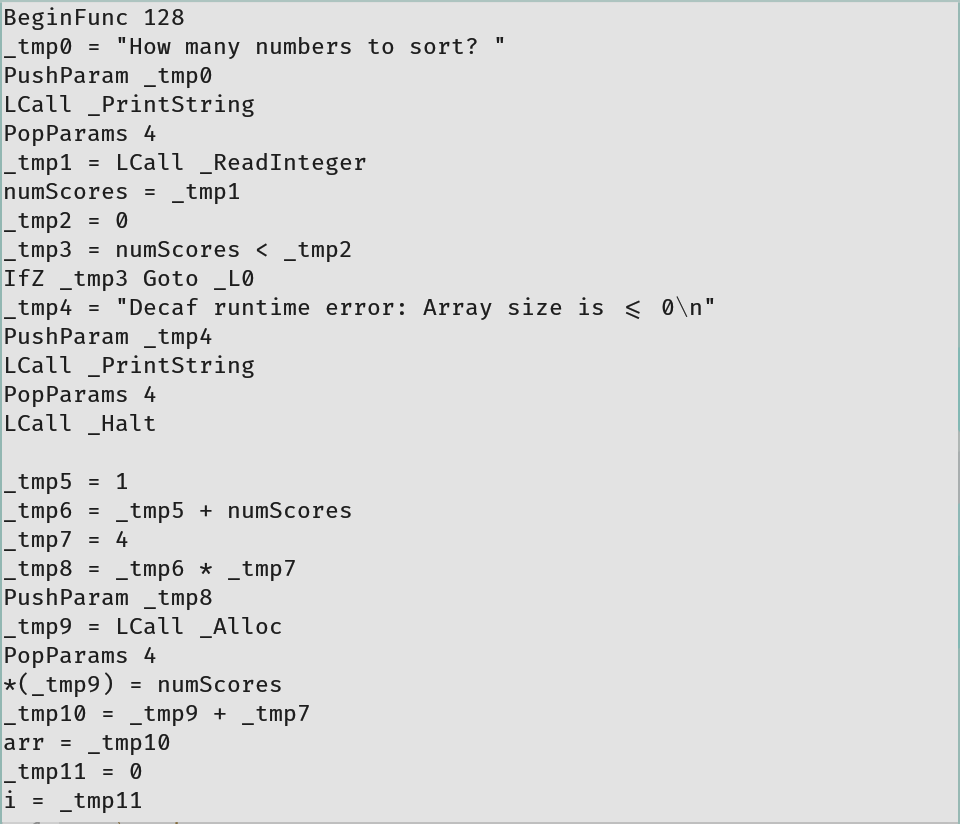
\includegraphics[width=0.82\linewidth]{tacprog.png}
    \caption{sort程序的TAC输出(部分)}
    \label{fig:tacprog}
\end{figure}


